\section*{Del 2}
\subsection*{Forsøgsopstilling}
Først anbringes en magnetomrører, som bruges til at røre puffer opløsningerne,
mens pH-elektroden kalibreres. Henover opsættes en dråbetæller,
som også skal kalibreres, med pH-elektroden ned langs.
Ovenfor placeres en autoburette fyldt op med en vis mængde titrator, i vores tilfælde ca. $15\ \unit{\milli\liter}\ \ce{NaOH}$.
Når alting er kalibreret kan man sætte titranten under, og da vi brugte autotitrering, så kan man bare trykke saml data.

\begin{figure}[h]
    \centering%
    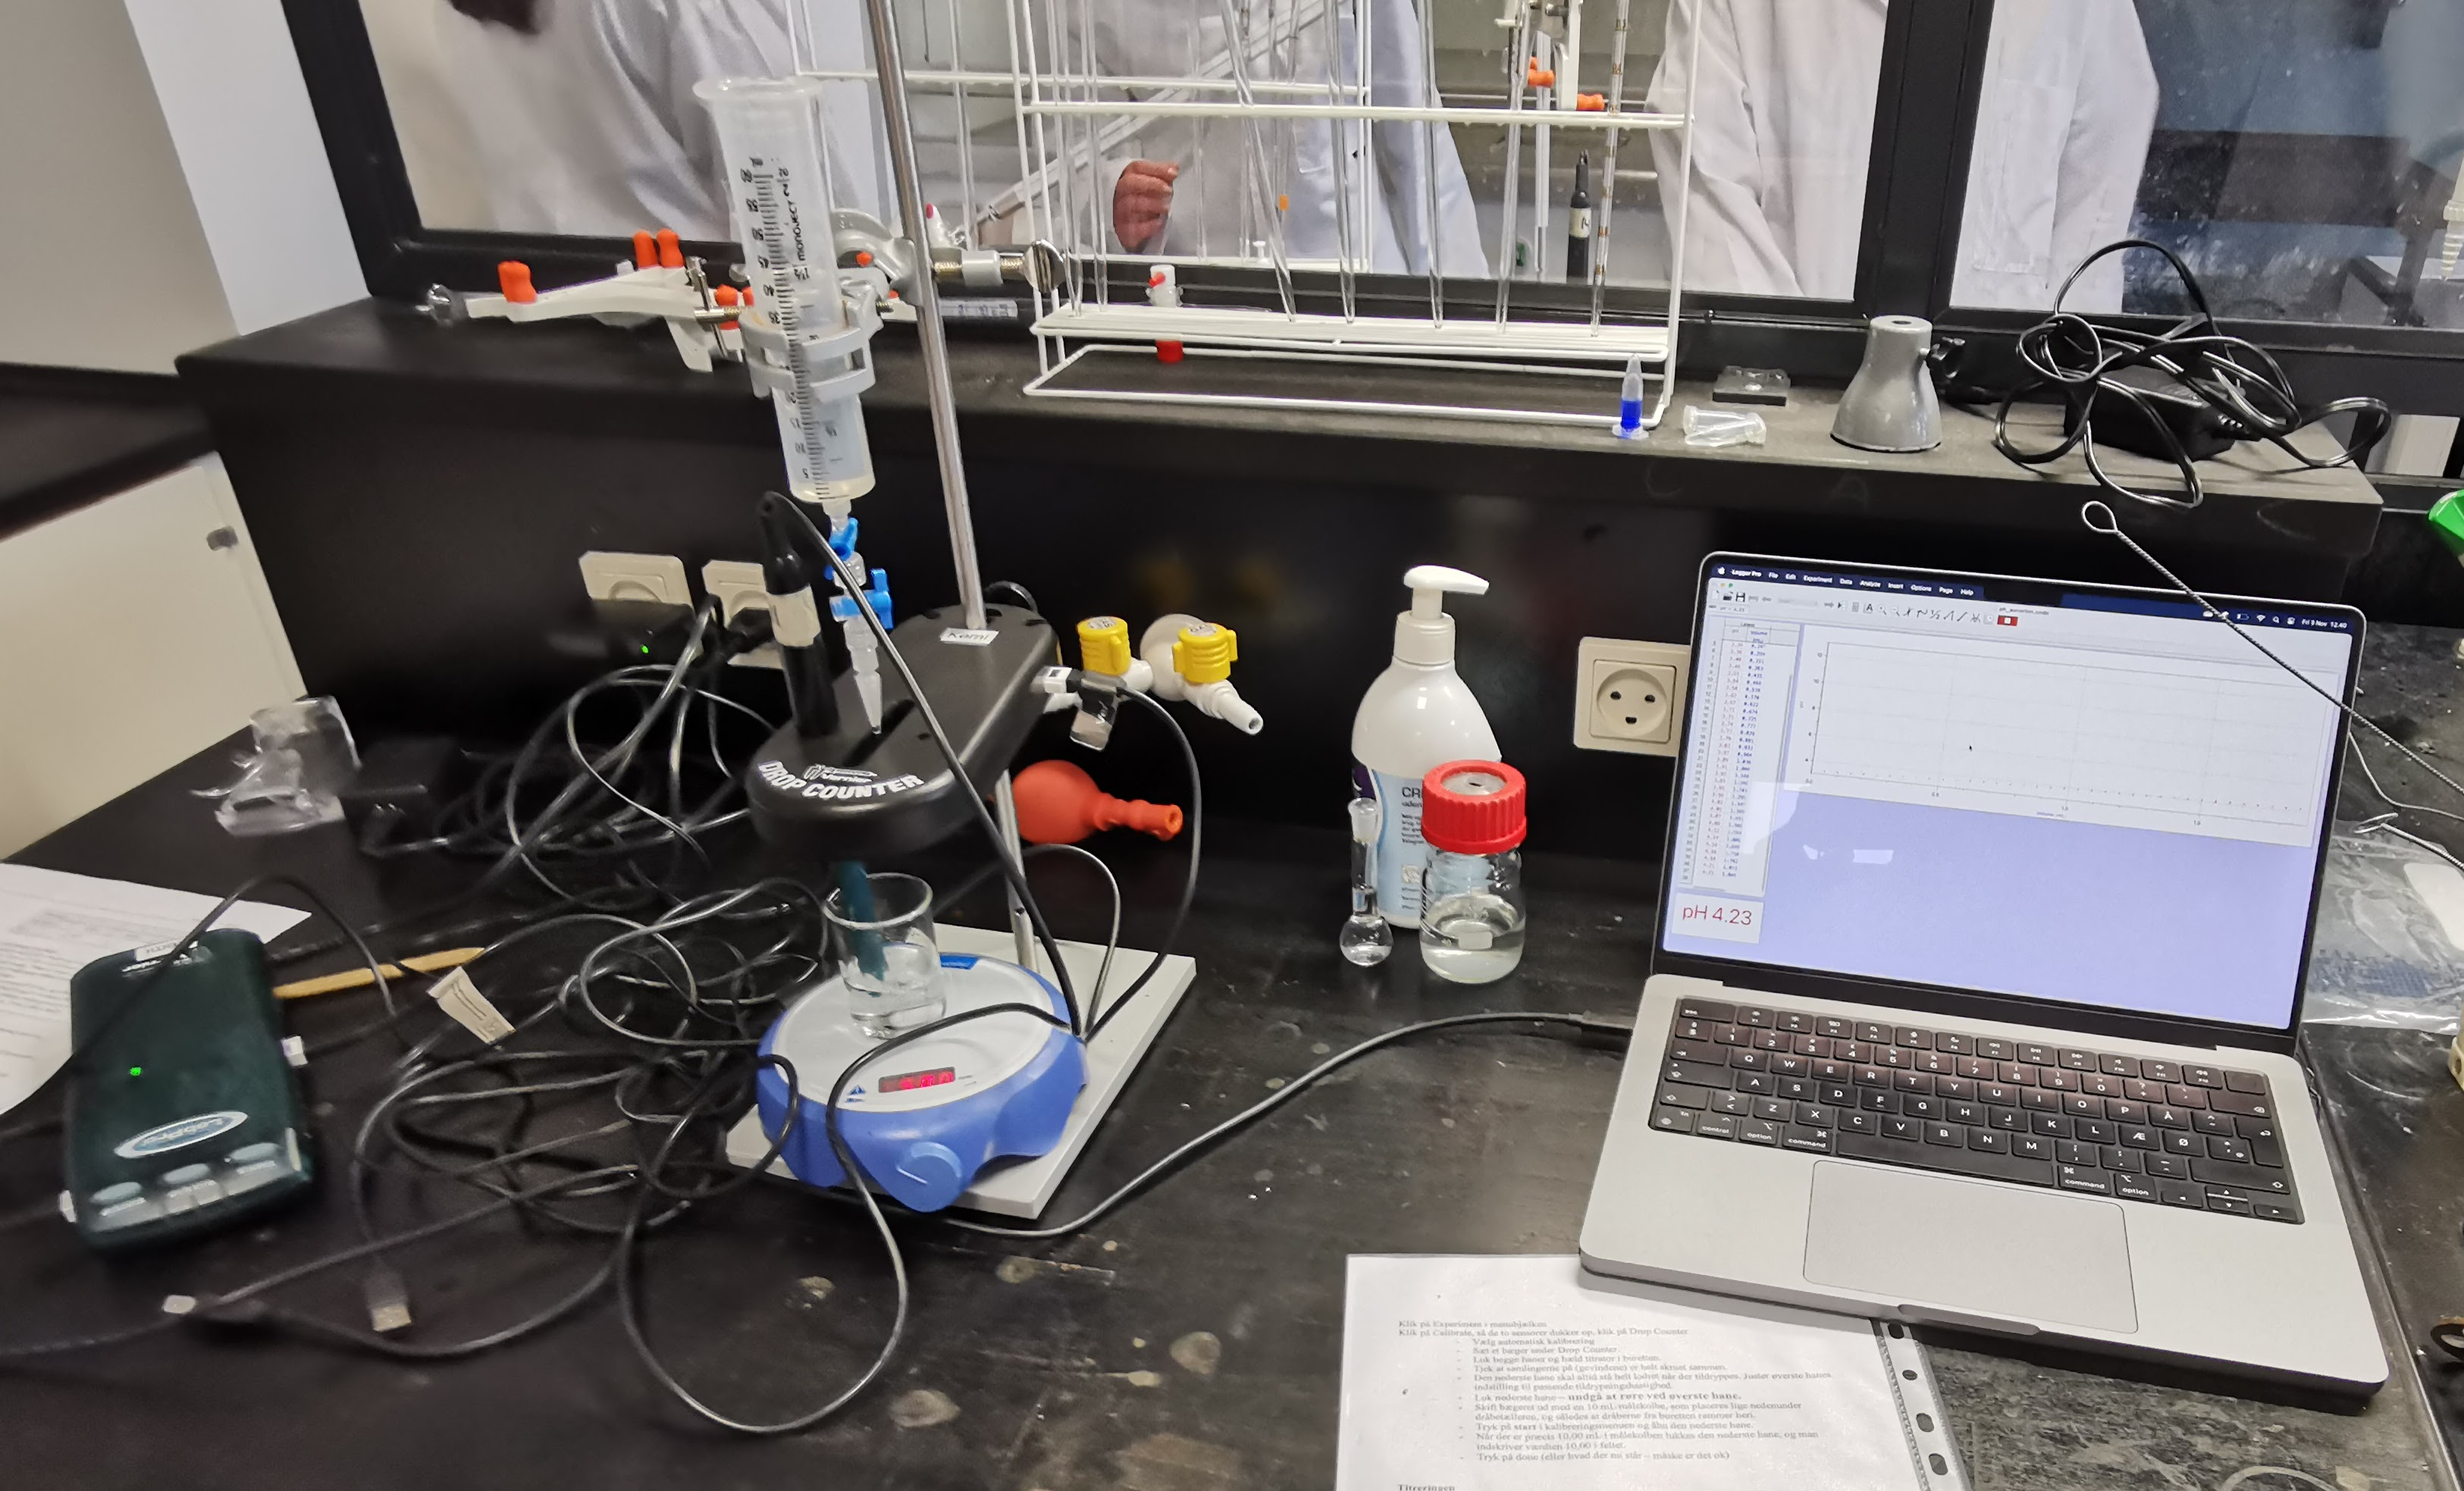
\includegraphics[width=8cm]{opstilling}
\end{figure}

\subsection*{Udførelse}
Vi opsatte jævnfør forsøgsopstillings afsnittet med titranten $0{,}1\ \textsc{m}$ ascorbinsyre og trykkede saml data.

\subsection*{Databehandling}
Titrering gav en flot titrerkurve, som ses nedenfor.
Midt på kurvens stejleste stykke kan vi aflæse pH-værdien for ækvivalenspunktet, som er markeret med rød på kurven, til at være ca. 8,7.
Da pH-værdien er 8,7, er det fordi,
at et af produkterne er \ce{C6H7O6-}, som er en amfolyt,
er mere en base end en syre.

\begin{tikzpicture}
    \begin{axis}[
        table/col sep=comma,
        width=.95\textwidth,
        height=0.4\textwidth,
        legend cell align=left,
        legend pos=north west,
        title=Titrering af ascorbinsyre,
        xlabel={$V(\ce{NaOH})/\unit{\milli\liter}$},
        ylabel={pH},
        grid,
        clip mode=individual
    ]
    \addplot[color=blue, mark=*]
    table[x index=1, y index=0, header=true] {del2/askorbinsyre.csv};

    % ækvivalenspunkt
    \node (mark) [label={0:{(6,2; 8,7)}},draw, red, circle, minimum size = 2pt, fill=red] 
    at (axis cs: 6.269, 8.78) {};
    % pks punkt
    \node (mark) [label={90:{(3,1; 4,6)}},draw, circle, minimum size = 2pt, fill=green, green] 
    at (axis cs: 3.109, 4.62) {};

    \end{axis}
\end{tikzpicture}

Derudover kan vi også aflæse $pK_s$ ud fra kurven, som er markeret med et grønt punkt, og det kan aflæses til ca. 4,6.
Grunden til, at vi kan aflæse $pK_s$ ud fra titrerkurven er,
at pufferligningen $pH=pK_s+\log\frac{1-x_s}{x_s}$ består af to led, det sidste led er,
hvor man tager $\log$ til syrebrøken, som giver procentdelen, der er syre.
Dvs.~at syrebrøken er $50\%$ halvvejs mod ækvivalenspunktet, derved giver leddet 0 og $pH=pK_s$.
Derfor går vi ud til halvdelen af ækvivalenspunktets x-værdi.

Til sidst kan vi udregne $K_s$ ved at gøre det omvendte af $-\log_{10}$:

\[
K_s=10^{-pK_s}=10^{-4{,}6}\ \textsc{m}=2{,}51 \cdot 10^{-5}\ \textsc{m}    
\]
